% !TEX program = xelatex
% Финальная презентация ВКР: AgentsSwarm
\documentclass[aspectratio=169,11pt]{beamer}

\usepackage{fontspec}
\usepackage[main=russian,english]{babel}
\usepackage{graphicx}
\usepackage{booktabs}
\usepackage{array}
\usepackage{tabularx}
\usepackage{pdfpages}
\usepackage{tikz}
\usetikzlibrary{calc,arrows.meta}

\graphicspath{{assets/}}

% Fonts: HSE Sans is not available in the current environment.
\setsansfont{Arial}
\setmainfont{Arial}
\setmonofont[Scale=0.86]{Courier New}
\usefonttheme{professionalfonts}

\definecolor{hseblue}{HTML}{0F2C68}
\definecolor{hselightblue}{HTML}{EAF0FA}
\definecolor{hsegray}{HTML}{667085}
\definecolor{hseline}{HTML}{D9E2F2}
\definecolor{hsegreen}{HTML}{1B7F5A}
\definecolor{hseorange}{HTML}{B95E04}
\definecolor{hseviolet}{HTML}{5B4BB2}

\setbeamercolor{normal text}{fg=black,bg=white}
\setbeamercolor{frametitle}{fg=hseblue,bg=white}
\setbeamercolor{footline}{fg=hsegray,bg=white}
\setbeamercolor{structure}{fg=hseblue}
\setbeamercolor{block title}{fg=white,bg=hseblue}
\setbeamercolor{block body}{fg=black,bg=hselightblue}
\setbeamerfont{frametitle}{series=\bfseries,size=\large}
\setbeamerfont{title}{series=\bfseries,size=\Large}
\setbeamerfont{subtitle}{size=\normalsize}
\setbeamerfont{footline}{size=\scriptsize}
\setbeamertemplate{navigation symbols}{}
\setbeamertemplate{itemize item}{\color{hseblue}\raisebox{0.12ex}{\scriptsize$\blacktriangleright$}}
\setbeamertemplate{itemize subitem}{\color{hseblue}\scriptsize$\bullet$}
\setlength{\parindent}{0pt}

\newcommand{\maintotal}{18}
\newcommand{\slidenumbertext}{\insertframenumber/\maintotal}

\setbeamertemplate{frametitle}{%
  \vspace{0.12cm}%
  \begin{beamercolorbox}[wd=\paperwidth,leftskip=0.55cm,rightskip=0.55cm,ht=0.48cm,dp=0.16cm]{frametitle}
    \insertframetitle
  \end{beamercolorbox}%
  \begin{tikzpicture}[remember picture,overlay]
    \draw[hseline,line width=0.6pt]
      ([xshift=0.55cm,yshift=-0.78cm]current page.north west) --
      ([xshift=-0.55cm,yshift=-0.78cm]current page.north east);
  \end{tikzpicture}%
  \vspace{-0.15cm}%
}

\setbeamertemplate{footline}{%
  \begin{beamercolorbox}[wd=\paperwidth,leftskip=0.55cm,rightskip=0.55cm,ht=0.32cm,dp=0.16cm]{footline}
    AgentsSwarm: кооперативное восприятие и LLM-оркестрация автономного роя
    \hfill \slidenumbertext
  \end{beamercolorbox}%
}

\newcommand{\thinrule}{\textcolor{hseline}{\rule{\linewidth}{0.5pt}}}

\newcommand{\metriccard}[3]{%
  \begin{minipage}[t]{0.31\linewidth}
    \begin{beamercolorbox}[wd=\linewidth,sep=0.12cm,center]{block body}
      {\color{hseblue}\bfseries\Large #1}\par
      \vspace{0.03cm}
      {\bfseries #2}\par
      \vspace{0.03cm}
      {\scriptsize\color{hsegray}#3}
    \end{beamercolorbox}
  \end{minipage}
}

\newcommand{\smallmetric}[3]{%
  \begin{minipage}[t]{0.23\linewidth}
    \begin{beamercolorbox}[wd=\linewidth,sep=0.10cm,center]{block body}
      {\color{hseblue}\bfseries\large #1}\par
      {\scriptsize #2}\par
      {\tiny\color{hsegray}#3}
    \end{beamercolorbox}
  \end{minipage}
}

\newcommand{\columnmetric}[3]{%
  \begin{beamercolorbox}[wd=\linewidth,sep=0.10cm,center]{block body}
    {\color{hseblue}\bfseries\large #1}\par
    {\scriptsize #2}\par
    {\tiny\color{hsegray}#3}
  \end{beamercolorbox}
}

\newcommand{\keybox}[2]{%
  \begin{beamercolorbox}[wd=\linewidth,sep=0.14cm]{block body}
    {\color{hseblue}\bfseries #1}\par
    \vspace{0.04cm}
    {\small #2}
  \end{beamercolorbox}
}

\newcommand{\tightkeybox}[2]{%
  \begin{beamercolorbox}[wd=0.98\linewidth,sep=0.09cm]{block body}
    {\color{hseblue}\bfseries\small #1}\par
    \vspace{0.02cm}
    {\scriptsize #2}
  \end{beamercolorbox}
}

\newcommand{\sectiontag}[1]{%
  {\scriptsize\bfseries\color{hsegray}\MakeUppercase{#1}}\par\vspace{0.06cm}
}

\newcounter{presfigure}
\newcounter{prestable}

\newcommand{\figcaption}[1]{%
  \refstepcounter{presfigure}%
  \vspace{0.05cm}%
  {\scriptsize\color{hsegray}Рисунок~\thepresfigure~\textemdash{} #1}\par
}

\newcommand{\tablecaption}[1]{%
  \refstepcounter{prestable}%
  {\scriptsize\color{hsegray}Таблица~\theprestable~\textemdash{} #1}\par
  \vspace{0.07cm}%
}

\title{Организация кооперативного восприятия сцены в группе автономных агентов на основе обмена визуальной информацией}
\subtitle{Многоагентная робототехническая платформа AgentsSwarm}
\author{Вольхин Данил Федорович}
\institute{Факультет компьютерных наук\\Исследование и предпринимательство в искусственном интеллекте}
\date{Москва, 2026}

\begin{document}

% 1

\includepdf[pages=1,pagecommand={\thispagestyle{empty}\addtocounter{framenumber}{1}},width=\paperwidth]{Титульный слайд.pdf}

% 2
\begin{frame}{Предметная область и термины}
  \sectiontag{Контекст работы}
  {\large\bfseries Работа находится на стыке multi-robot systems, fleet management,
  LLM-агентов и цифрового двойника.}
  \vspace{0.28cm}

  \begin{columns}[T,onlytextwidth]
    \begin{column}{0.49\textwidth}
      \begin{minipage}[t][2.10cm][t]{\linewidth}
        \keybox{AMR/AGV-флот}{группа мобильных роботов, которым нужны общая карта, статусы и согласованные маршруты}
      \end{minipage}
      \vspace{0.14cm}
      \keybox{VDA5050}{промышленный формат обмена между fleet manager и роботами}
    \end{column}
    \begin{column}{0.49\textwidth}
      \begin{minipage}[t][2.10cm][t]{\linewidth}
        \keybox{MCP}{стандартный tool-интерфейс между LLM-агентами и внешними сервисами}
      \end{minipage}
      \vspace{0.14cm}
      \keybox{Digital twin}{Isaac Sim и ROS\,2 позволяют проверить маршрут до физического внедрения}
    \end{column}
  \end{columns}

  \vspace{0.22cm}
  \begin{beamercolorbox}[wd=\linewidth,sep=0.13cm]{block body}
    \small Предмет работы не низкоуровневое управление колесами, а архитектура,
    которая переводит смысловую задачу человека в исполнимый контур миссий.
  \end{beamercolorbox}
\end{frame}

% 3
\begin{frame}{Проблема и мотивация}
  \begin{columns}[T,onlytextwidth]
    \begin{column}{0.50\textwidth}
      \sectiontag{Ключевой разрыв}
      {\Large\bfseries Одиночный робот видит локальную ситуацию,\\
      но решение часто должно менять поведение всей группы.}
      \vspace{0.35cm}

      \scriptsize
      Существующие fleet management системы надежно диспетчеризуют миссии,
      но не дают высокоуровневого семантического планирования и интерфейса
      на естественном языке.
    \end{column}
    \begin{column}{0.46\textwidth}
      \keybox{Локальное восприятие}{камера, лидар и вычисления ограничены одним роботом}
      \vspace{0.16cm}
      \keybox{Разрозненные контуры}{симуляция, VDA5050, LLM и UI обычно живут отдельно}
      \vspace{0.16cm}
      \keybox{Нет реактивной оркестрации}{сложно быстро перестроить миссии роя по наблюдениям}
    \end{column}
  \end{columns}
\end{frame}

% 4
\begin{frame}{Исследовательский разрыв}
  \begin{columns}[T,onlytextwidth]
    \begin{column}{0.31\textwidth}
      \keybox{Cooperative perception}{алгоритмы дают обмен признаками и детекциями, но редко интегрируются с промышленным fleet management}
    \end{column}
    \begin{column}{0.31\textwidth}
      \keybox{VDA5050 и fleet management}{дают надежную диспетчеризацию, но требуют формальных API-команд}
    \end{column}
    \begin{column}{0.31\textwidth}
      \keybox{LLM-агенты}{умеют планировать и вызывать инструменты, но нуждаются в ограниченном исполнимом контуре}
    \end{column}
  \end{columns}
  \vspace{0.42cm}
  \begin{beamercolorbox}[wd=\linewidth,sep=0.18cm]{block body}
    \textbf{\color{hseblue}Вклад работы:}
    воспроизводимая интеграция LLM-слоя, MCP-инструментов, VDA5050,
    ROS 2 и цифрового двойника Isaac Sim в одну исполнимую архитектуру.
  \end{beamercolorbox}
\end{frame}

% 5
\begin{frame}{Цель и задачи}
  \sectiontag{Цель работы}
  \begin{beamercolorbox}[wd=\linewidth,sep=0.14cm]{block body}
    \normalsize Создать AgentsSwarm: программный комплекс, который переводит
    запрос на естественном языке в скоординированные миссии группы роботов.
  \end{beamercolorbox}
  \vspace{0.22cm}

  \sectiontag{Как цель декомпозирована}

  \begin{columns}[T,onlytextwidth]
    \begin{column}{0.49\textwidth}
      \begin{minipage}[t][1.60cm][t]{\linewidth}
        \tightkeybox{Архитектура}{8 компонентов: интерфейс, Orchestrator, vLLM, MCP-слой и роботический контур}
      \end{minipage}
      \vspace{0.11cm}
      \tightkeybox{Агентное планирование}{Router, Planner, PlanRunner и агенты для карт, роботов и маршрутов}
    \end{column}
    \begin{column}{0.49\textwidth}
      \begin{minipage}[t][1.60cm][t]{\linewidth}
        \tightkeybox{Интеграционные протоколы}{3 асинхронных MCP-сервера, VDA5050-совместимые заказы и ROS 2}
      \end{minipage}
      \vspace{0.11cm}
      \tightkeybox{Проверка и оптимизация}{контур в Isaac Sim, pytest/smoke-проверки и дистилляция SmolVLA}
    \end{column}
  \end{columns}

  \vspace{0.16cm}
  {\scriptsize\color{hsegray}
  Объект: многоагентная робототехническая система; методы: системный анализ,
  микросервисное проектирование, симуляционный эксперимент.}
\end{frame}

% 6
\begin{frame}{Требования и ограничения}
  \sectiontag{Что должна выдерживать архитектура}
  \begin{columns}[T,onlytextwidth]
    \begin{column}{0.32\textwidth}
      \begin{minipage}[t][1.80cm][t]{\linewidth}
        \tightkeybox{Естественный язык}{пользователь формулирует задачу без ручной сборки API-вызовов}
      \end{minipage}
      \vspace{0.12cm}
      \tightkeybox{VDA5050}{исполнение оформляется как совместимый заказ миссии}
    \end{column}
    \begin{column}{0.32\textwidth}
      \begin{minipage}[t][1.80cm][t]{\linewidth}
        \tightkeybox{MCP}{LLM вызывает ограниченный каталог инструментов}
      \end{minipage}
      \vspace{0.12cm}
      \tightkeybox{ROS\,2 + Isaac Sim}{проверка идет в симуляционном роботическом контуре}
    \end{column}
    \begin{column}{0.32\textwidth}
      \begin{minipage}[t][1.80cm][t]{\linewidth}
        \tightkeybox{Streaming}{статусы, tool-вызовы и ответ видны пользователю}
      \end{minipage}
      \vspace{0.12cm}
      \tightkeybox{Воспроизводимость}{компоненты разнесены как сервисы и фиксируются версиями}
    \end{column}
  \end{columns}
  \vspace{0.28cm}
  \begin{beamercolorbox}[wd=\linewidth,sep=0.14cm]{block body}
    \small Ограничение принципиально: LLM не помещается в servo-loop робота;
    она работает на уровне плана и инструментов, а выполнение остаётся в роботическом контуре.
  \end{beamercolorbox}
\end{frame}

% 7
\begin{frame}{Используемые технологии}
  \sectiontag{Стек программного проекта}
  \begin{columns}[T,onlytextwidth]
    \begin{column}{0.49\textwidth}
      \begin{minipage}[t][1.90cm][t]{\linewidth}
        \keybox{Backend и агенты}{Python, FastAPI, OpenAI Agents SDK, FastMCP, pytest}
      \end{minipage}
      \vspace{0.10cm}
      \keybox{Frontend и данные}{React, Chakra UI, Celery, Redis Streams, RabbitMQ, PostgreSQL, MinIO}
    \end{column}
    \begin{column}{0.49\textwidth}
      \begin{minipage}[t][1.90cm][t]{\linewidth}
        \keybox{LLM-инференс}{vLLM Service, Qwen2.5-Instruct, OpenAI-compatible API, Data Parallel на 2\,×\,Tesla V100}
      \end{minipage}
      \vspace{0.10cm}
      \keybox{Роботический контур}{NVIDIA Isaac Sim, ROS\,2 Jazzy, Nav2, rosbridge, Mosquitto, VDA5050}
    \end{column}
  \end{columns}
  \vspace{0.20cm}
  \begin{beamercolorbox}[wd=\linewidth,sep=0.13cm]{block body}
    \small Стек выбран под разделение ролей: веб-интерфейс, агентное планирование,
    LLM-инференс и роботическое исполнение связаны через REST, WebSocket, MCP и MQTT.
  \end{beamercolorbox}
\end{frame}

% 8
\begin{frame}{Инфраструктура развёртывания}
  \vspace{0.08cm}
  \small
  \renewcommand{\arraystretch}{1.2}
  \tablecaption{Технические характеристики вычислительной инфраструктуры}
  \begin{tabular}{@{}>{\bfseries\color{hseblue}\raggedright\arraybackslash}m{2.80cm}>{\raggedright\arraybackslash}m{1.95cm}>{\raggedright\arraybackslash}m{4.05cm}>{\raggedright\arraybackslash}m{3.45cm}@{}}
    \toprule
    \textbf{Назначение} & \textbf{Провайдер} & \textbf{Конфигурация} & \textbf{Сервисы} \\
    \midrule
    Симуляция & Selectel & 4 vCPU, 16 ГБ RAM, RTX 4090 24 ГБ VRAM & Isaac Sim, ROS 2, Mission Control \\
    \midrule
    Микросервисы & Selectel & 4 vCPU, 8 ГБ RAM, 128 ГБ SSD & Interface, Orchestrator, Mission Dispatch, Redis, RabbitMQ, MinIO, PostgreSQL \\
    \midrule
    LLM-кластер & MTS Cloud & 2 узла $\times$ Tesla V100-PCIE 32 ГБ VRAM & vLLM Data Parallel, Qwen2.5-Instruct \\
    \bottomrule
  \end{tabular}
  \vspace{0.22cm}
  
  \begin{beamercolorbox}[wd=\linewidth,sep=0.12cm]{block body}
    \small \textbf{\color{hseblue}Сетевые контуры:}
    HTTP/REST между сервисами, WebSocket для стриминга, MQTT для VDA5050,
    gRPC для vLLM Data Parallel.
  \end{beamercolorbox}
\end{frame}

% 9
\begin{frame}{Идея}
  \sectiontag{Ключевой принцип}
  {\large\bfseries LLM не управляет роботом напрямую: LLM планирует поверх ограниченного набора инструментов.}
  \vspace{0.20cm}

  % Fixed-size tikzpicture scaled to fit the text column.
  % Native width ≈ 14 cm → scale 0.86 → rendered ≈ 12.0 cm ≈ \linewidth.
  \scalebox{0.86}{%
  \begin{tikzpicture}[
    box/.style={draw=hseblue, line width=0.8pt, rounded corners=2pt, align=center,
                minimum height=0.90cm, text width=2.35cm, font=\small},
    arrow/.style={-{Latex[length=1.8mm]}, line width=0.85pt, draw=hseblue},
    back/.style={-{Latex[length=1.8mm]}, line width=0.75pt, draw=hsegray, dashed}
  ]
    \node[box] (user)  at (0,    0) {Естественный\\язык};
    \node[box] (llm)   at (3.00, 0) {Агент};
    \node[box] (mcp)   at (6.00, 0) {Инструменты};
    \node[box] (vda)   at (9.00, 0) {VDA5050};
    \node[box] (robot) at (12.00,0) {Симуляция};

    \draw[arrow] (user)  -- (llm);
    \draw[arrow] (llm)   -- (mcp);
    \draw[arrow] (mcp)   -- (vda);
    \draw[arrow] (vda)   -- (robot);

    % feedback arc stays below boxes; label on the line
    \draw[back]
      (robot.south) -- ++(0,-0.70)
      -- node[below, font=\scriptsize, text=hsegray, fill=white, inner sep=1pt,
              midway] {обратная связь исполнения}
      ($(llm.south)+(0,-0.70)$) -- (llm.south);
  \end{tikzpicture}%
  }

  \vspace{0.10cm}

  \begin{columns}[T,onlytextwidth]
    \begin{column}{0.30\textwidth}
      \tightkeybox{Совместимость}{MCP, VDA5050, ROS~2, OpenAI-compatible API}
    \end{column}
    \begin{column}{0.30\textwidth}
      \tightkeybox{Наблюдаемость}{шаги плана и tool-вызовы попадают в поток событий}
    \end{column}
    \begin{column}{0.30\textwidth}
      \tightkeybox{Воспроизводимость}{компоненты изолированы как сервисы}
    \end{column}
  \end{columns}
\end{frame}

% 10
\begin{frame}{Общая архитектура AgentsSwarm}
  \vspace{-0.10cm}
  \begin{center}
  \begin{tikzpicture}[
    layerbox/.style={draw=hseline, line width=0.6pt, rounded corners=2pt, fill=hselightblue, inner sep=4pt},
    component/.style={draw=hseblue, line width=0.7pt, rounded corners=2pt, fill=white,
                      align=center, minimum height=0.68cm, text width=3.00cm, font=\scriptsize},
    service/.style={component, draw=hseviolet},
    robot/.style={component, draw=hsegreen},
    queue/.style={component, draw=hseorange},
    arrow/.style={-{Latex[length=1.8mm]}, draw=hseblue, line width=0.7pt},
    event/.style={-{Latex[length=1.8mm]}, draw=hsegray, line width=0.6pt, dashed},
    layername/.style={font=\small\bfseries, text=hseblue, align=center}
  ]
    % layer backgrounds (width 3.6cm each, gap 0.5cm, centres at 1.9, 6.0, 10.1)
    \node[layerbox, minimum width=3.60cm, minimum height=4.10cm] at (1.90,2.05) {};
    \node[layerbox, minimum width=3.60cm, minimum height=4.10cm] at (6.00,2.05) {};
    \node[layerbox, minimum width=3.60cm, minimum height=4.10cm] at (10.10,2.05) {};

    \node[layername] at (1.90,3.95)  {Пользователь};
    \node[layername] at (6.00,3.95)  {Планирование};
    \node[layername] at (10.10,3.95) {Исполнение};

    \node[component] (user)    at (1.90,3.22) {Пользователь\\естественный язык};
    \node[component] (ui)      at (1.90,2.05) {Interface\\React + FastAPI};
    \node[queue]     (streams) at (1.90,0.88) {RabbitMQ / Redis\\queue + events};

    \node[component] (orch) at (6.00,3.22) {Orchestrator\\Router / Planner / PlanRunner};
    \node[service]   (vllm) at (6.00,2.05) {vLLM Service\\Qwen2.5 · 2\,×\,V100};
    \node[component] (mcp)  at (6.00,0.88) {3 MCP-сервера\\MC / Dispatch / ROS\,2};

    \node[robot] (mc)  at (10.10,3.22) {Mission Control\\Behavior Tree};
    \node[robot] (md)  at (10.10,2.05) {Mission Dispatch\\VDA5050 / MQTT};
    \node[robot] (sim) at (10.10,0.88) {ROS\,2 + Isaac Sim\\Carter robots};

    \draw[arrow] (user) -- (ui);
    \draw[arrow] (ui)   -- (streams);
    \draw[arrow] (ui.east)  -- (orch.west);
    \draw[arrow] (orch) -- (vllm);
    \draw[arrow] (orch) -- (mcp);
    \draw[arrow] (mcp.east) -- (mc.west);
    \draw[arrow] (mcp.east) -- (md.west);
    \draw[arrow] (mcp.east) -- (sim.west);
    \draw[arrow] (mc)  -- (md);
    \draw[arrow] (md)  -- (sim);
    \draw[event] (streams.east) -- (orch.west);
  \end{tikzpicture}
  \end{center}
  \vspace{-0.02cm}
  \begin{columns}[T,onlytextwidth]
    \begin{column}{0.32\textwidth}
      \columnmetric{8}{самостоятельных компонентов}{UI, Orchestrator, vLLM, MCP, ROS\,2, Isaac Sim, Mission Control/Dispatch, SmolVLA}
    \end{column}
    \begin{column}{0.32\textwidth}
      \columnmetric{3}{логических слоя}{восприятие, планирование, исполнение}
    \end{column}
    \begin{column}{0.32\textwidth}
      \columnmetric{4}{протокола связи}{REST, WebSocket, MQTT, MCP}
    \end{column}
  \end{columns}
\end{frame}

% 11
\begin{frame}{Сквозной маршрут команды}
  \vspace{0.05cm}
  \begin{center}
  \begin{tikzpicture}[
    rstep/.style={draw=hseblue, line width=0.75pt, rounded corners=2pt, fill=white,
                  align=center, minimum height=1.0cm, text width=1.70cm, font=\scriptsize},
    tool/.style={rstep, fill=hselightblue},
    exec/.style={rstep, draw=hsegreen, fill=white},
    arrow/.style={-{Latex[length=1.8mm]}, draw=hseblue, line width=0.75pt},
    event/.style={-{Latex[length=1.8mm]}, draw=hsegray, line width=0.65pt, dashed}
  ]
    \node[rstep] (s1) at (0.0, 1.85) {Запрос\\на языке};
    \node[rstep] (s2) at (1.95,1.85) {Interface\\task};
    \node[tool]  (s3) at (3.90,1.85) {Orchestrator\\план};
    \node[tool]  (s4) at (5.85,1.85) {MCP\\tools};
    \node[exec]  (s5) at (7.80,1.85) {Mission\\Dispatch};
    \node[exec]  (s6) at (9.75,1.85) {VDA5050\\MQTT};
    \node[exec]  (s7) at (11.70,1.85){Carter\\Isaac Sim};

    \foreach \a/\b in {s1/s2,s2/s3,s3/s4,s4/s5,s5/s6,s6/s7}
      \draw[arrow] (\a) -- (\b);

    \node[draw=hsegray, rounded corners=2pt, fill=hselightblue,
          align=center, text width=6.20cm, font=\scriptsize,
          inner sep=4pt] (events) at (5.85,0.18)
      {Redis Streams + WebSocket\\возвращают статусы, tool-события и финальный ответ};

    \draw[event] (s7.south) .. controls +(0,-0.90) and +(2.4,0.65) .. (events.east);
    \draw[event] (events.west) .. controls +(-2.4,0.65) and +(0,-0.90) .. (s2.south);
  \end{tikzpicture}
  \end{center}
  \vspace{0.06cm}
  \begin{beamercolorbox}[wd=\linewidth,sep=0.14cm]{block body}
    \small
    Пользовательский запрос превращается в план, затем в вызовы MCP-инструментов,
    затем в VDA5050 order через Mission Dispatch и MQTT-контур робота в Isaac Sim.
  \end{beamercolorbox}
\end{frame}

% 12
\begin{frame}{Orchestrator: агентная архитектура}
  \vspace{0.05cm}
  \begin{center}
  \resizebox{\linewidth}{!}{%
  \begin{tikzpicture}[
    main/.style={draw=hseblue, line width=0.9pt, rounded corners=2pt, fill=white,
                 align=center, minimum height=0.90cm, text width=2.60cm, font=\normalsize},
    agent/.style={main, fill=hselightblue, text width=2.10cm, minimum height=0.78cm},
    tool/.style={main, draw=hsegreen, text width=2.60cm},
    arrow/.style={-{Latex[length=2mm]}, draw=hseblue, line width=0.8pt},
    bus/.style={draw=hseblue, line width=0.7pt}
  ]
    \node[main, text width=2.20cm] (task)    at (0,    2.85) {Task\\+ context};
    \node[main] (router)  at (2.90, 2.85) {Router\\класс запроса};
    \node[main] (planner) at (5.80, 2.85) {Planner\\план шагов};
    \node[main] (runner)  at (8.70, 2.85) {PlanRunner\\исполнение};
    \node[tool] (mcp)     at (11.60,2.85) {MCP tools\\robotic APIs};

    \draw[arrow] (task)    -- (router);
    \draw[arrow] (router)  -- (planner);
    \draw[arrow] (planner) -- (runner);
    \draw[arrow] (runner)  -- (mcp);

    \node[font=\small, text=hsegray, fill=white, inner sep=1.5pt]
      at (5.80, 1.95) {handoff к специализированным агентам};

    \draw[bus] (0,1.72) -- (11.60,1.72);

    \draw[arrow] (runner.south) -- (8.70,1.72);

    \node[agent] (ri)  at (0,    0.78) {RobotInfo};
    \node[agent] (ma)  at (2.90, 0.78) {MapAnalyst};
    \node[agent] (nav) at (5.80, 0.78) {Navigation};
    \node[agent] (sw)  at (8.70, 0.78) {Swarm\\Coordinator};
    \node[agent] (gen) at (11.60,0.78) {General};

    \foreach \a/\x in {ri/0, ma/2.90, nav/5.80, sw/8.70, gen/11.60}
      \draw[arrow] (\x,1.72) -- (\a.north);
  \end{tikzpicture}%
  }
  \end{center}
  \vspace{0.02cm}
  \begin{columns}[T,onlytextwidth]
    \begin{column}{0.32\textwidth}
      \columnmetric{Router}{классификация запроса}{выбор handoff-направления}
    \end{column}
    \begin{column}{0.32\textwidth}
      \columnmetric{Planner}{декомпозиция миссии}{шаги, зависимости, роботы}
    \end{column}
    \begin{column}{0.32\textwidth}
      \columnmetric{PlanRunner}{исполнение}{агенты и MCP-инструменты}
    \end{column}
  \end{columns}
\end{frame}

% 13
\begin{frame}{MCP-слой: стандартный интерфейс к роботическому контуру}
  \begin{columns}[T,onlytextwidth]
    \begin{column}{0.56\textwidth}
      \vspace{0.10cm}
      \resizebox{\linewidth}{!}{%
      \begin{tikzpicture}[
        box/.style={draw=hseblue, line width=0.75pt, rounded corners=2pt, fill=white,
                    align=center, minimum height=0.72cm, text width=2.30cm, font=\scriptsize},
        mcp/.style={box, fill=hselightblue},
        backend/.style={box, draw=hsegreen},
        arrow/.style={-{Latex[length=1.7mm]}, draw=hseblue, line width=0.7pt}
      ]
        \node[box, text width=2.60cm] (orch) at (3.60,3.55) {Orchestrator\\MCP clients};
        \node[mcp] (mcpmc)  at (0.95,2.15) {\texttt{mission\vphantom{p}}\\\texttt{-control-mcp}};
        \node[mcp] (mcpmd)  at (3.60,2.15) {\texttt{mission\vphantom{p}}\\\texttt{-dispatch-mcp}};
        \node[mcp] (mcpros) at (6.25,2.15) {\texttt{ros-msp}\\stdio / WS};

        \node[backend] (mc)  at (0.95,0.72) {Mission Control\\карта · robots\\waypoints};
        \node[backend] (md)  at (3.60,0.72) {Mission Dispatch\\миссии\\очередь};
        \node[backend] (ros) at (6.25,0.72) {ROS\,2\\topics\\services};

        \draw[arrow] (orch) -- (mcpmc);
        \draw[arrow] (orch) -- (mcpmd);
        \draw[arrow] (orch) -- (mcpros);
        \draw[arrow] (mcpmc)  -- (mc);
        \draw[arrow] (mcpmd)  -- (md);
        \draw[arrow] (mcpros) -- (ros);
      \end{tikzpicture}%
      }
    \end{column}
    \begin{column}{0.41\textwidth}
      \sectiontag{Зоны ответственности}
      \small
      \begin{itemize}
        \item \texttt{mission-control-mcp}: карта, waypoint-граф, статусы.
        \item \texttt{mission-dispatch-mcp}: отправка и мониторинг миссий.
        \item \texttt{ros-msp}: ROS\,2 topics через rosbridge WebSocket.
      \end{itemize}
    \end{column}
  \end{columns}
  \vspace{0.52cm}
  \keybox{Почему это важно}{Оркестратор не зависит от конкретной реализации роботического контура и работает через tool-интерфейс.}
\end{frame}

% 14
\begin{frame}{Роботический контур: Isaac Sim, ROS 2 и VDA5050}
  \begin{columns}[T,onlytextwidth]
    \begin{column}{0.45\textwidth}
      \centering
      \vspace{0.00cm}
      \begin{tikzpicture}[
        box/.style={draw=hseblue, line width=0.75pt, rounded corners=2pt, fill=white,
                    align=center, minimum height=0.68cm, text width=4.05cm, font=\small},
        robot/.style={box, draw=hsegreen},
        broker/.style={box, draw=hseorange},
        arrow/.style={-{Latex[length=1.7mm]}, draw=hseblue, line width=0.72pt},
        state/.style={-{Latex[length=1.5mm]}, draw=hsegray, line width=0.62pt, dashed}
      ]
        \node[box]    (mc)   at (2.10,4.95) {Mission Control\\route + Behavior Tree};
        \node[box]    (md)   at (2.10,3.75) {Mission Dispatch\\mission queue};
        \node[broker] (mqtt) at (2.10,2.55) {Mosquitto\\VDA5050 / MQTT};
        \node[robot]  (ros)  at (2.10,1.35) {ROS\,2 Jazzy\\Nav2 + rosbridge};
        \node[robot]  (sim)  at (2.10,0.15) {Isaac Sim\\Carter robots};

        \draw[arrow] (mc) -- (md);
        \draw[arrow] (md) -- (mqtt);
        \draw[arrow] (mqtt) -- (ros);
        \draw[arrow] (ros) -- (sim);

        \draw[state] (sim.east) -- ++(0,0) |- node[pos=0.25, right, font=\tiny, text=hsegray]
          {state} (mc.east);
      \end{tikzpicture}\par
      \figcaption{Схема интеграции Isaac Sim, ROS\,2 и VDA5050 в симуляционном контуре}
    \end{column}
    \begin{column}{0.51\textwidth}
      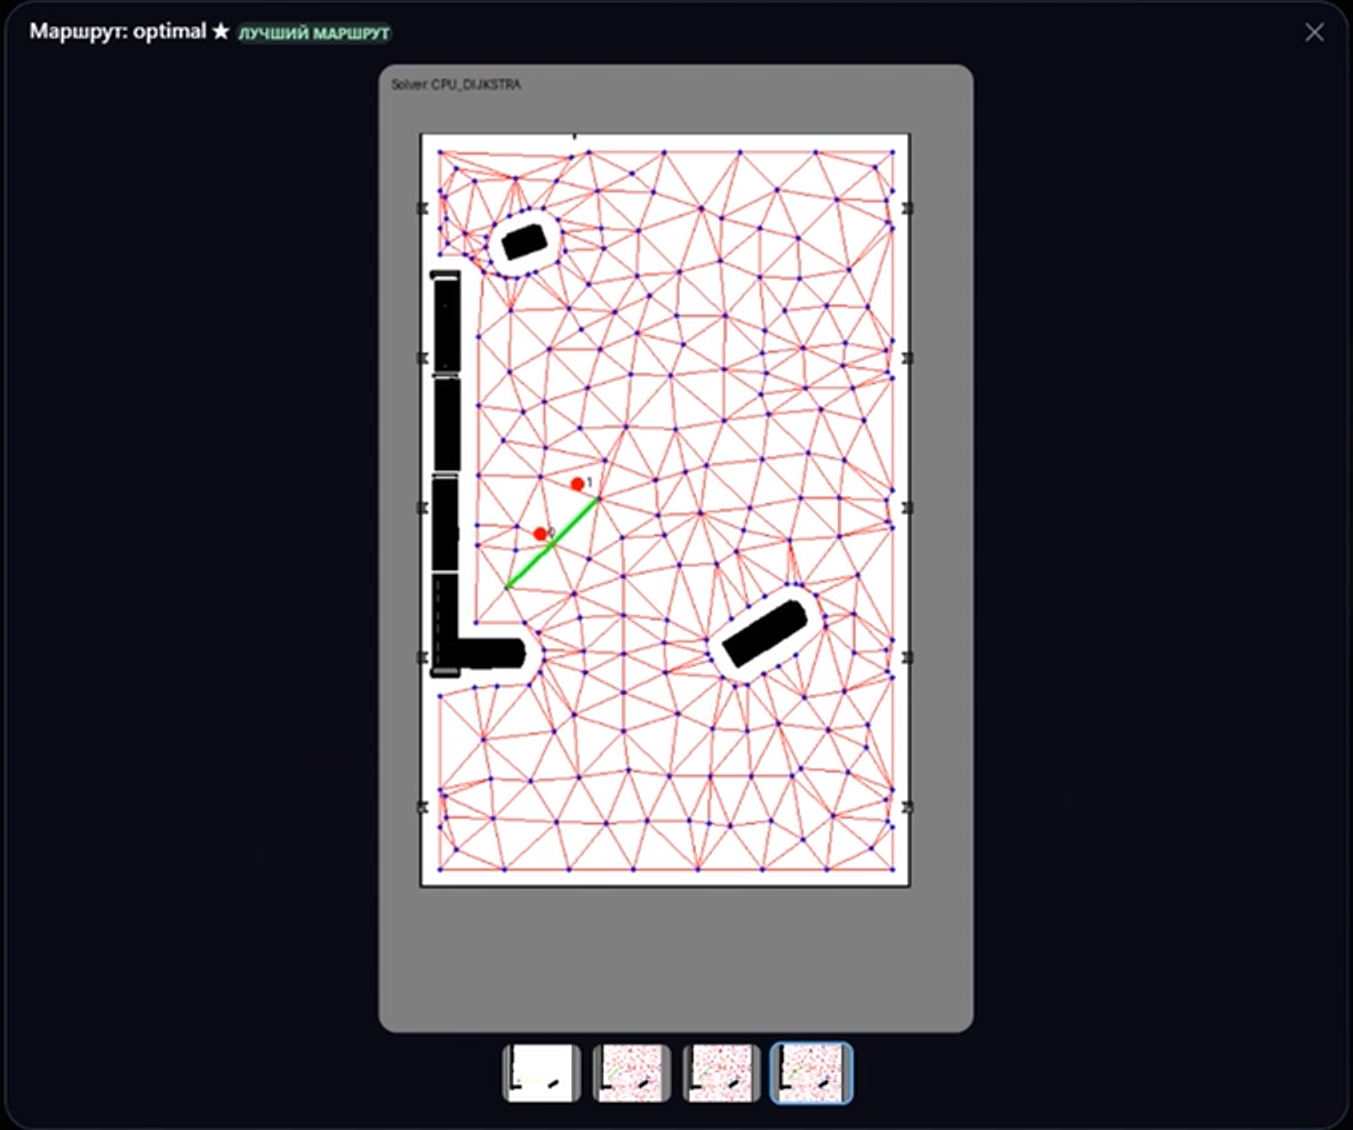
\includegraphics[width=\linewidth,height=0.68\textheight,keepaspectratio]{fig_3_2_map_waypoints.png}\par
      \figcaption{Occupancy map и waypoint graph сцены Carter Warehouse}
    \end{column}
  \end{columns}
\end{frame}

% 15
\begin{frame}{Потоковая модель событий}
  \vspace{0.10cm}
  \begin{center}
  \scalebox{0.86}{%
  \begin{tikzpicture}[
    state/.style={draw=hseblue, line width=0.85pt, rounded corners=2pt, fill=white,
                  align=center, minimum height=0.95cm, text width=2.60cm, font=\small},
    stream/.style={state, fill=hselightblue, text width=2.80cm},
    arrow/.style={-{Latex[length=1.9mm]}, draw=hseblue, line width=0.8pt},
    event/.style={-{Latex[length=1.9mm]}, draw=hsegray, line width=0.65pt, dashed}
  ]
    \node[state]                 (pending) at (0.0,  0) {\texttt{pending}\\задача создана};
    \node[state]                 (running) at (3.20, 0) {\texttt{running}\\агенты + tools};
    \node[state, draw=hsegreen]  (done)    at (6.40, 0) {\texttt{completed}\\ответ готов};
    \node[state, draw=hseorange] (err)     at (3.20,-1.55) {\texttt{error}\\остановка};

    \node[stream] (redis) at (9.80,  0) {Redis Stream\\event log};
    \node[stream] (ws)    at (9.80,-1.55) {WebSocket\\live UI};

    \draw[arrow] (pending) -- (running);
    \draw[arrow] (running) -- (done);
    \draw[arrow] (running) -- (err);

    \draw[event] (pending.north) -- ++(0,0.55) -| (redis.north);
    \draw[event] (running.north) -- ++(0,0.55) -| (redis.north);
    \draw[event] (done.east)     -- (redis.west);
    \draw[event] (err.east)      -- ++(1.0,0) |- (ws.west);

    \draw[arrow] (redis) -- (ws);
  \end{tikzpicture}%
  }
  \end{center}
  \vspace{0.08cm}
  \begin{columns}[T,onlytextwidth]
    \begin{column}{0.48\textwidth}
      \keybox{Жизненный цикл}{\textit{pending} $\to$ \textit{running} $\to$ \textit{completed} или \textit{error}}
    \end{column}
    \begin{column}{0.48\textwidth}
      \keybox{Наблюдаемость}{события \texttt{stream\_chunk}, \texttt{routing\_event}, \texttt{tool\_event}, \texttt{agent\_reply}}
    \end{column}
  \end{columns}
\end{frame}

% 16
\begin{frame}{Демонстрация интерфейса}
  \begin{columns}[T,onlytextwidth]
    \begin{column}{0.33\textwidth}
      
\includegraphics[width=\linewidth,height=0.58\textheight,keepaspectratio]{qr_demo.pdf}\par
      \figcaption{QR-код на видео-демо}
    \end{column}
    \begin{column}{0.65\textwidth}
      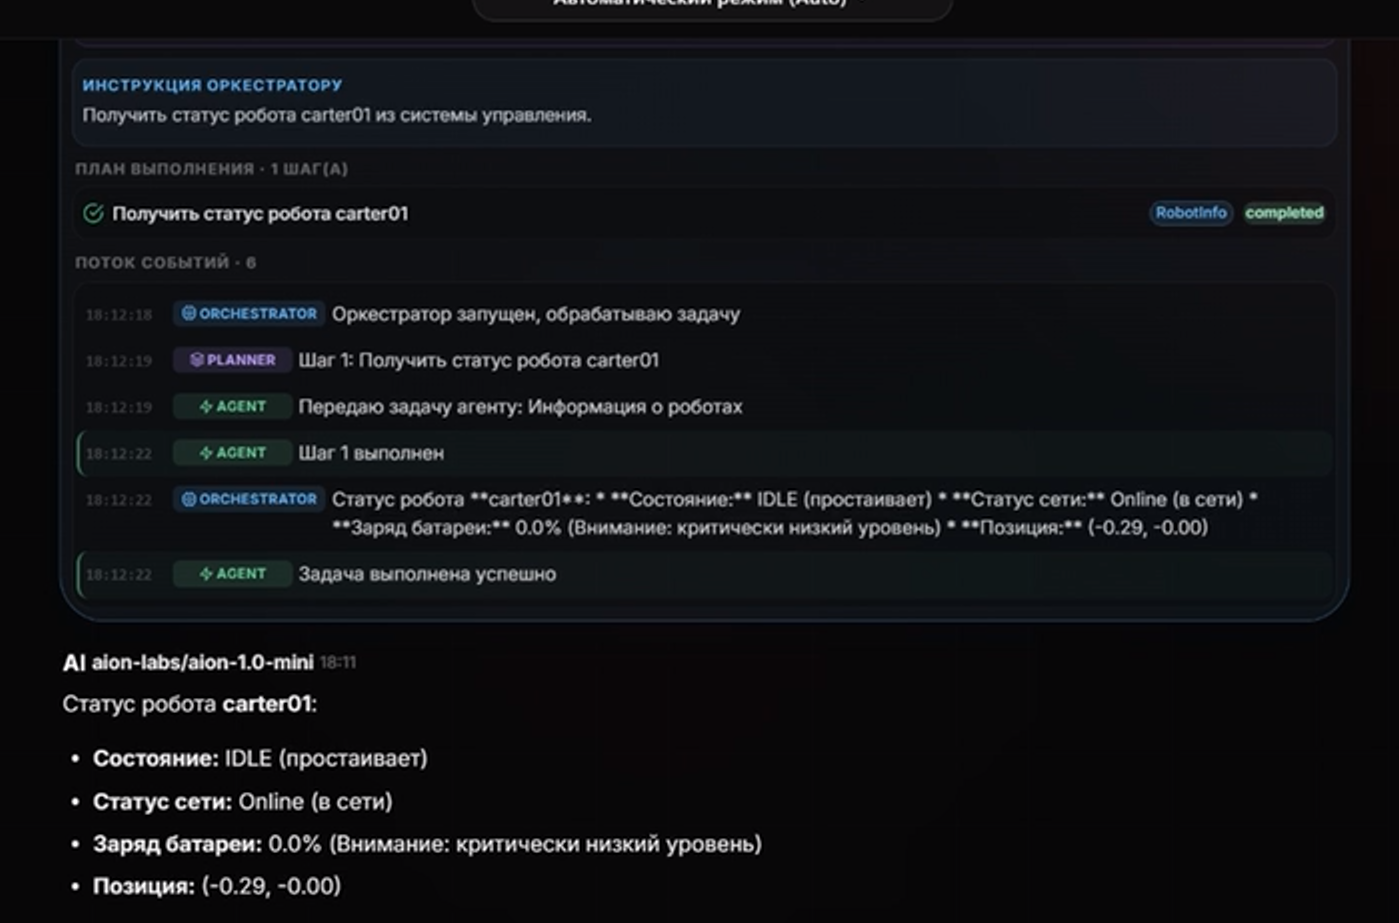
\includegraphics[width=\linewidth,height=0.82\textheight,keepaspectratio]{fig_3_10_trace.png}\par
      \figcaption{Экран TracePanel: трассировка агентного маршрута}
    \end{column}
  \end{columns}
\end{frame}

% 17
\begin{frame}{SmolVLA: перспектива — кастомный VDA5050 action-handler}
  \vspace{-0.06cm}
  \begin{columns}[T,onlytextwidth]
    \begin{column}{0.36\textwidth}
      \centering
      \begin{tikzpicture}[
        box/.style={draw=hseblue, line width=0.6pt, rounded corners=1pt, fill=white,
                    align=center, minimum height=0.44cm, text width=2.68cm, font=\tiny},
        nav/.style={box, fill=hselightblue},
        vla/.style={box, draw=hsegreen, fill=green!8},
        done/.style={box, draw=hsegreen},
        arrow/.style={-{Latex[length=1.3mm]}, draw=hseblue, line width=0.55pt,
                      shorten <=1pt, shorten >=1pt}
      ]
        \node[box]  (orch) at (1.42,3.82) {LLM-оркестратор\\создаёт миссию};
        \node[box]  (mc)   at (1.42,3.02) {Mission Control\\order + \texttt{vla\_action}};
        \node[nav]  (nav)  at (1.42,2.22) {Навигация\\к action-узлу};
        \node[vla]  (vla)  at (1.42,1.42) {vla\_action handler\\SmolVLA on Jetson};
        \node[done] (task) at (1.42,0.62) {Задача выполнена\\(захват объекта)};
        \node[done] (cont) at (1.42,-0.18){Продолжение\\навигационной миссии};

        \draw[arrow] (orch.south) -- (mc.north);
        \draw[arrow] (mc.south)   -- (nav.north);
        \draw[arrow] (nav.south)  -- (vla.north);
        \draw[arrow] (vla.south)  -- (task.north);
        \draw[arrow] (task.south) -- (cont.north);
      \end{tikzpicture}
      \vspace{0.03cm}

      {\tiny\color{hsegray}Рисунок~5~\textemdash{} Навигация~+~бортовая автономность}
    \end{column}%
    \begin{column}{0.61\textwidth}
      \scriptsize\textbf{\color{hseblue}Идея:} VDA5050 order содержит поле \texttt{actions} в узлах маршрута; тип \texttt{vla\_action} запускает локальный инференс SmolVLA вместо навигационной команды. Робот останавливается, выполняет задание, продолжает миссию.
      \vspace{0.05cm}

      \scriptsize\textbf{\color{hseblue}Целевая платформа:} NVIDIA Jetson Orin Nano (8\,ГБ VRAM). Оптимизация SmolVLA делает бортовой инференс достижимым.
      \vspace{0.05cm}

      \tiny
      \setlength{\tabcolsep}{2.8pt}
      \renewcommand{\arraystretch}{1.12}
      \tablecaption{Ключевые результаты оптимизации SmolVLA}
      \begin{tabularx}{\linewidth}{@{}>{\bfseries\color{hseblue}\raggedright\arraybackslash}m{1.85cm}
                                      >{\raggedleft\arraybackslash}m{1.05cm}
                                      >{\raggedleft\arraybackslash}m{1.05cm}
                                      >{\raggedright\arraybackslash}X@{}}
        \toprule
        Метрика & Teacher & Student & Изменение \\
        \midrule
        Параметры   & 450M          & $\approx$1M    & $\times$443 сжатие \\
        VRAM        & 6{,}0\,ГБ     & <0{,}5\,ГБ    & $\times$12 снижение \\
        Латентность & 450\,мс       & 18\,мс         & $\times$25 ускорение \\
        $R^2$       & 0{,}841       & 0{,}826        & $-$1{,}8\% \\
        \bottomrule
      \end{tabularx}
      \vspace{0.05cm}

      \scriptsize\textbf{\color{hseblue}Результат:} AgentsSwarm расширяется от «доставить в точку~B» до «доставить и выполнить физическое задание»~--- от NL-запроса до бортовой манипуляции.
      \vspace{0.04cm}

      {\tiny\color{hsegray}\textbf{Примечание:} эксперимент~--- \texttt{lerobot/libero}; перенос на Jetson Orin Nano требует отдельного профилирования.}
    \end{column}
  \end{columns}
\end{frame}

% 18
\begin{frame}{Полученные результаты}
  \tiny
  \renewcommand{\arraystretch}{1.02}
  \tablecaption{Компоненты AgentsSwarm: срезы разработки и результаты}
  \begin{tabularx}{\linewidth}{@{}>{\bfseries\color{hseblue}\raggedright\arraybackslash}m{2.25cm}>{\raggedright\arraybackslash}m{2.10cm}>{\raggedright\arraybackslash}X@{}}
    \toprule
    \textbf{Модуль} & \textbf{Срез / объём} & \textbf{Результат} \\
    \midrule
    vLLM Service & v0.2.9, 32 коммита & Qwen2.5-Instruct развёрнут как OpenAI-compatible сервис на 2\,×\,Tesla V100. \\
    \midrule
    Ros2 контур & форки и настройка окружения & Mission Control/Dispatch, VDA5050/MQTT, ROS\,2 Jazzy исполняют миссию, а Isaac Sim реализует миссию в физической симуляции. \\
    \midrule
    MCP-серверы & 3 async-сервера & Orchestrator получает tool-интерфейс к Mission Control, Mission Dispatch и ros-msp. \\
    \midrule
    Orchestrator & v0.5.6, 61 коммит & Router классифицирует запрос, Planner строит план, PlanRunner исполняет его через агентов. \\
    \midrule
    Interface & v0.5.0, 168 коммитов & Пользователь ставит задачу, запускает агентный сценарий и видит поток выполнения в веб-интерфейсе. \\
    \midrule
    Тестирование & 66 тестов & Проверены ключевые сценарии Orchestrator; Interface закрыт route, WebSocket и smoke-проверками. \\
    \midrule
    SmolVLA Tools & v0.2.3, 6 коммитов & Показаны сжатие параметров, снижение VRAM и ускорение при падении $R^2$ на 1.8\%. \\
    \bottomrule
  \end{tabularx}
  \vspace{0.32cm}

  \begin{beamercolorbox}[wd=\linewidth,sep=0.12cm]{block body}
    \scriptsize\bfseries\color{hseblue}
    Итог: сквозной маршрут от естественного языка до исполнимой VDA5050-миссии
    собран, описан и проверен в симуляционном роботическом контуре.
  \end{beamercolorbox}
  \vspace{0.04cm}
  \begin{center}
    {\small\bfseries Спасибо за внимание. Готов ответить на вопросы.}
  \end{center}
\end{frame}

\appendix
\renewcommand{\slidenumbertext}{резерв}


\includepdf[pages=1,pagecommand={\thispagestyle{empty}},width=\paperwidth]{Последний слайд.pdf}

\end{document}
